\begin{figure}[h]
    \centering
    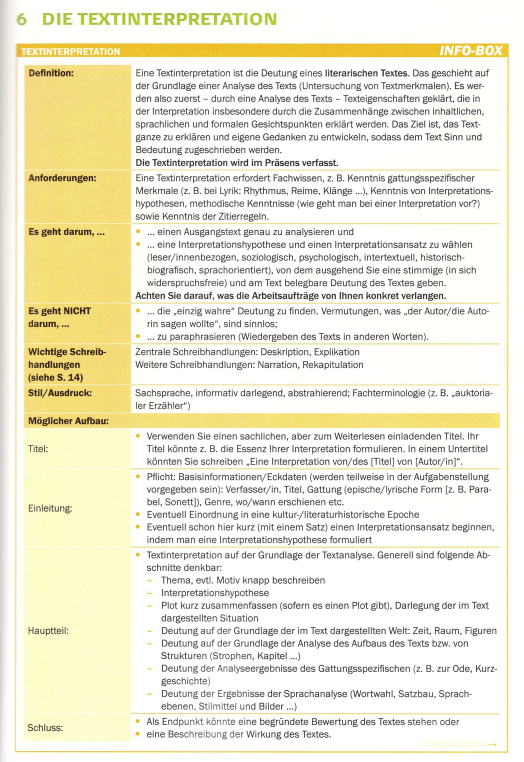
\includegraphics[scale=0.8]{./pics/Screenshot from 2023-02-06 12-31-18.png}
    \caption{Textinterpretation: Definition + Aufbau}
    \label{fig:impl:Textinterpretation1}
\end{figure}

\begin{figure}[h]
    \centering
    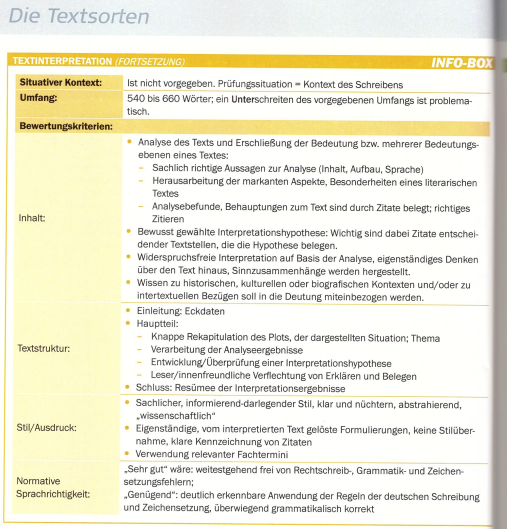
\includegraphics[scale=0.8]{./pics/Screenshot from 2023-02-06 12-31-28.png}
    \caption{Textinterpretation: Verfassen}
    \label{fig:impl:Textinterpretation2}
\end{figure}
\begin{figure}[h]
    \centering
    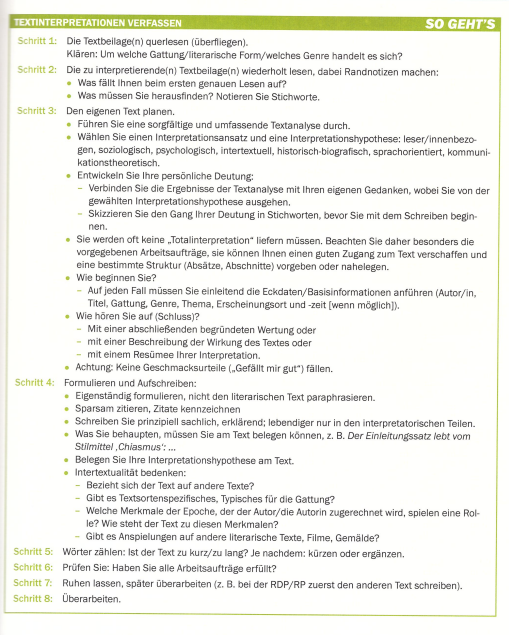
\includegraphics[scale=0.8]{./pics/Screenshot from 2023-02-06 12-32-23.png}
    \caption{Textinterpretation: Fortsetzung}
    \label{fig:impl:Textinterpretation3}
\end{figure}



\section{Mustertext}

\subsubsection{Nichts ist unpräziser als Gerechtigkeit }
Eine Interpretation von „Lieferung frei Haus“ von Günter Kunert 

In der Kurzgeschichte „Lieferung frei Haus“, die 1988 in „Arbeitstexte für den Deutschunterricht. Deutsche Kurzgeschichten 11. – 13. Schuljahr“ erschien, beschreibt Günter Kunert die Tücken einer Welt, in der absolute Gerechtigkeit herrscht, und stellt gleichzeitig die Frage, ob man einen Menschen für alle Folgen seines Handelns verantwortlich machen kann.  

Anfangs wird beschrieben, wie anonyme Lastwägen in der Dämmerung Holzkisten an verschiedenste Haushalte ausliefern. Dies geschieht auch im Haus, in dem Friedrich W. Schmall, der Hauptcharakter, wohnhaft ist. Im Vorbeigehen bemerkt er den Empfänger, der diese Lieferung voller Entsetzen entgegennimmt. Schmall wird schon bald von der Portiersfrau aufgeklärt, beim Inhalt der Kisten handle es sich um Leichen. Dieses absurde Vorkommnis wird ihm von der Bäckersfrau bestätigt, deren Mann ebenfalls eine Leiche in Empfang nehmen musste. Es handelt sich um eine Greisin, die dieser auf regennasser Straße mit seinem Auto tötete. Schmall kann sich einen Anflug von Freude über diese ausgleichende Gerechtigkeit nicht verkneifen. Auf der Straße trifft er auf eine Menschenmenge, die beobachtet, wie ein Ex-Soldat, der Deserteure erschoss, vierzig Kisten geliefert bekommt. Danach bekommt Schmall erstmals Zweifel an den Akteuren und der moralischen Rechtfertigung hinter diesen Lieferungen. Als er seine Verlobte besuchen will, bekommt auch sie eine solche Lieferung. Er flüchtet, ohne mit ihr zu sprechen. Als er sie später darauf anspricht, rechtfertigt sie sich, doch er flüchtet wieder. Die Geschichte endet damit, dass auch Friedrich W. Schmall eine Holzkiste geliefert bekommt, die seine Verlobte beinhaltet. Sie konnte den Verlust ihres Mannes nicht verkraften und nahm sich das Leben.  

Die Kurzgeschichte ist aus der Perspektive eines personalen Erzählers geschrieben, der die Handlung linear wiedergibt und stets im Präteritum bleibt. Sprachlich fallen besonders die Beschreibungen der Personen auf, besonders die Beschreibungen der Empfänger der Holzkisten im Moment der Übergabe sind sehr lebhaft und vermitteln ein fast schon überzeichnetes Bild des Entsetzens. So vergleicht er etwa das Gesicht eines Empfängers mit einer „bleichen, großen Blase“, die mit „zwei schwarzen Knöpfen“ besetzt sei (Z 28 – 30). Der groteske Effekt der Lieferung einer Leiche an einen normalen Haushalt wird so nochmals verstärkt, da auch die Empfänger als leichenähnlich beschrieben werden.  Sprachliche Besonderheiten sind auch in der letzten Szene vorhanden, in der Friedrich W. Schmall selbst zum Empfänger wird.  Der Autor verlängert die Zeit künstlich, und die Erzählzeit wird um ein Vielfaches länger als die erzählte Zeit. Auch werden die handelnden Personen als teilnahmslos dargestellt, so etwa Friedrich W. Schmall, der „ohne das Gefährt zu beachten“ (Z188) sein Haus betritt, oder auch die Lieferanten, „aus deren Unbeweglichkeit ihn die Augen reglos anglotzten“ (Z196). Dieser leblose Ablauf wird durch die lebhafte Überzeugung der Hauptfigur, dass es sich bei der Lieferung um einen Irrtum handeln müsse, unterbrochen. Als er allerdings seine Verlobte in der Kiste erkennt, resigniert er nach „einer von den kleineren Ewigkeiten“ (Z214), was nochmals eine Zeitdehnung darstellt.  

In der Kurzgeschichte wird eine absolute moralische Kraft in eine anderweitig normale Welt eingeführt. Diese absolute moralische Kraft besteht aus den Lieferanten der Kisten beziehungsweise ihren Auftraggebern, die entscheiden, wer Schuld am Tod der Verstorbenen hat. Diese Entscheidungen werden von amtlicher Seite getroffen (Z.64), und von niemanden in Frage gestellt. Besonders nicht von den Empfängern der Kisten, da diese oftmals zu schockiert über die Schuldzuweisung sind, und diese möglichst vor der Öffentlichkeit verbergen möchten. Auch für beobachtende Passanten ist es leichter, die Empfänger als Schuldige darzustellen, als mit ihnen zu sympathisieren, da so die Annäherung an eventuelle Mörder argumentativ verteidigt werden müsste. Dieser Mechanismus schützt die Kräfte hinter den Auslieferungen und ihre Entscheidungen vor jeglichen öffentlichen Verurteilungen. Dadurch ähnelt das beschriebene System autoritären Regimen, in denen Regierungen oder Behörden Entscheidungen treffen können, die einzelne Bürger stark negativ betreffen, ohne selbst Konsequenzen fürchten zu müssen. Friedrich W. Schmall zeigt hierzu im Verlauf der Geschichte drei typische Einstellungen der Bevölkerung zu diesen Umständen. Anfangs ist er noch erfreut darüber, dass dem Bäcker Gerechtigkeit widerfährt (Z72). Später stellt er allerdings die Möglichkeit fest, dass auch Irrtümer geschehen könnten und dass solche Schuldentscheidungen nie wirklich gerecht gefällt werden können. Schließlich erfährt er am eigenen Leib, wie es ist, die Schuld am Tod eines Mitmenschen zugesprochen zu bekommen. Bemerkenswert ist hierbei auch, dass die exekutierenden Personen ihre Aufgabe ohne Gewissensbisse erledigen, und die Liste der angeblichen Mörder als normal abzuarbeitende Aufgabe betrachten (Z. 219). Dieses Abweisen von Schuld ist wiederum ein typisches Kennzeichen von autoritären Strukturen. 

Diese Diskussion der Schuld in all ihren Facetten, insbesondere in autoritären Strukturen, wie sie im Laufe der Geschichte immer wieder auftrat, gelingt dem Autor in dieser Kurzgeschichte äußerst prägnant. Er stellt Fragen, die auch in unserer heutigen Gesellschaft noch nicht gelöst sind, und die jeder Leser für sich selbst beantworten muss. 

\section{Eigener Text}
\subsubsection{Die Toten lassen grüßen }

In der Kurzgeschichte “Lieferung frei Haus”, welche im Jahr 1988 von Günter Kunert veröffentlicht wurde, geht es um einen sonderbaren Vorgang, bei dem eines Tages viele Menschen hölzerne Kisten zugestellt bekommen. Friedrich Schmall, der Protagonist, beobachtet eines Tages in seiner Straße mehr Lastwägen als gewöhnlich unterwegs sind und allerlei Särge mit Leichen an manche Personen zugestellt werden. Erst ist er noch ganz verwundert, ob das Gesagte stimmen möge, doch der Besuch beim Bäcker gibt ihm dann Gewissheit. Aufgrund eines Platzmangels auf dem Friedhof bekommt jede Person, welche einen Menschen getötet hatte, die Leiche desjenigen zugestellt. An dem Tag nach dem Besuch bei des Bäckers Frau bekommt dann auch seine Frau Felicia Wirwark die Leiche eines Kindes zugestellt. Und obwohl er sicher ist, noch nie einem Menschen solch ein Leid angetan zu haben, bekommt auch er am Ende der Geschichte solch ein mysteriöses kistenartiges Paket. Und zu seinem Schock liegt dort drinnen ganz still und unbeweglich, seine Frau Felicia Wirwark. Mit diesem Plot endet der Text. 

 

Die Erzählzeit der Geschichte beträgt etwa 10 – 15 Minuten, während die erzählte Zeit etwa 3 Tage umfasst. Der Text ist in der Er-Erzählung verfasst, und der Autor verwendet nur Hypotaxen und Parataxen (Z.3-11) “Keineswegs auffiel jedenfalls nicht zuerst, dass nach allabendlichem Aufkommen der Dunkelheit wie auch im Dämmer einsamer Morgen diese Lastwagen, die bis dahin scheinbar ziellos durch die Straßen gekurvt, plötzlich vor dem oder jenem Haus stehen bleiben, um etwas Kastenförmiges, Kistenartiges, Hölzern-Kubisches aus sich zu entlassen, womit der Fahrer und Gehilfen gewöhnlich übereilig im Haustor verschwanden.” Viele seiner Sätze bestehen aus solchen Verschachtelungen, welche den Text teilweise sehr schwer zu lesen machen. Was auch auffällig ist, sind die Umschreibungen für das Wort Sarg. Bereits in der neunten Zeile werden die Wörter “Kastenförmiges”, ”Kistenartiges”, ”und "Hölzern-Kubisches” verwendet, um das Wort “Sarg” zu umschreiben. Damit verharmlost der Autor die Tatsache, dass es sich um Menschenleichen handelt, und hält die Spannung am Anfang noch sehr niedrig. Erst nach und nach wird es klarer, was Friedrich Schmall da eigentlich beobachtet. Was auch auffällig ist, sind die vielen Metaphern, welche der Autor in seinem Text benützt. “Wulstige und geborstenen Lippen” (Zeile 65), “hüpfendes Glucksen” (Zeile 73), “aufgesperrter Mund” (Zeile 149), “von einer Blutwelle dunkelrot gefärbt” (Zeile 166), um nur wenige Beispiele der sehr bildhaften Erzählung zu nennen. 

Doch was könnte der Autor damit gemeint haben? Welchen Grund könnte es geben, dass der Protagonist am Ende seiner Erzählung die Leiche seiner eigenen Frau geschickt bekommt? Für mich sind das alles Anspielungen auf die NS-Zeit. Nach den Schilderungen des Erzählers, nach der Beschreibung der Außenwelt und des Lebensstandards spielt die Geschichte in der Nachkriegszeit. Die Wirtschaft hat sich erholt, und die Menschen führen ein geregeltes Leben. Doch mit einem Schlag kommt die Vergangenheit wieder zurück. Bei manchen, weil sie bei einem Unfall Menschen tödlich verletzten, bei Frau Felicia Wirwark, weil sie damals das Uneheliche Kind mit Friedrich Schmall abgetrieben hat. Der Obersekretär hatte im Krieg 40 Menschen auf dem Gewissen, und auch ihn holt seine Vergangenheit im Forme der Särge wieder ein. Die Zeile 97 (“Man weiß es nicht genau, was die Belieferten machen. Ein Mann ist gestern festgenommen worden, als er Leichenteile in eine Mülltonne stopfte”) kann man so deuten, dass es den Betroffenen nicht möglich ist, ihre Vergangenheit zu vergessen. Hinter sich zu lassen. Aber was hat es mit den ganzen anderen Leichen auf sich, welche sich die Leute nicht erklären können? Auch das ist meiner Meinung nach auf den Krieg zurückzuführen. 
Viele Menschen, vor allem Juden, sind damals ums Leben gekommen, weil sie von ihren Nachbarn verraten oder ausgeliefert worden. Es wurden damals auch viele Menschen hingerichtet, weil ihnen niemand geholfen hat und jeder nur auf sich schaute. Und da man dadurch zuließ, dass so viele Menschen getötet wurden, kommen in der Geschichte die ganzen Leichen der unschuldigen Opfer der Nazis genau zu den Leuten, welche sie damals verraten hatten.	 


\section{Formulierungshilfen}   
Einleitung
\begin{compactitem}
    \item Der vorliegende Sachtext „(Titel)“ von (Autor) aus dem Jahr (Entstehungsjahr) handelt von.../ thematisiert... 
    \item Im vorliegenden Sachtext mit dem Titel „(Titel)“ von (Autor) veröffentlicht am (Entstehungsdatum) in (Verlag/ Herausgeber) geht es um... 
    \item Das zentrale These/ Intention/ Absicht des Autors scheint ... zu sein. (Deutungshypothese) 
\end{compactitem}
Hauptteil
\begin{compactitem}
    \item Der Text lässt sich in folgende Sinnesabschnitte einteilen.../ gliedern... Der erste Abschnitt beginnt in Zeile... und endet in Zeile... Er thematisiert/ benennt/ zählt... auf/ fokussiert... 
    \item Zu Beginn wird beschrieben.../ Der Autor beginnt mit der Beschreibung... 
    \item Im zweiten Abschnitt fährt der Autor fort mit der Schilderung der.... 
    \item Abschließend fasst er zusammen, dass.../ schlussfolgert er, dass.../ betont er... 
\end{compactitem}

Schlussteil
\begin{compactitem}
    \item Zusammenfassend ist festzuhalten, dass... 
    \item Meine anfangs aufgestellt Deutungshypothese hat sich (nicht) bestätigt, denn... / hat sich in dem Punkt bestätigt werden, dass.../ kann erweitert werden um... 
    \item Am Ende meiner Ausführungen komme ich zu dem Schluss, dass der Autor eine eher restriktive/ polarisierende / strikte/ liberale/ gemäßigte Haltung zu dem Thema... einnimmt. 
    \item Abschließend ist daher anzunehmen, dass der Autor ... 
    \item Als Fazit meiner Analyse lässt sich festhalten, dass... 
\end{compactitem}